\documentclass[final]{article}

\usepackage{APS360}
\usepackage[utf8]{inputenc}
\usepackage[T1]{fontenc}
\usepackage{hyperref}
\usepackage{url}
\usepackage{booktabs}
\usepackage{amsfonts}
\usepackage{nicefrac}
\usepackage{microtype}
\usepackage{xcolor}
\usepackage{graphicx}
\usepackage{tikz}
\usetikzlibrary{positioning, arrows.meta}

\title{Mini-VLM: A Pure RWKV Vision-Language Model\\for Efficient Visual Question Answering}

\author{%
  Oliver Petrovic \\
  1008923042, oliver.petrovic@mail.utoronto.ca\\
  \url{https://github.com/Olipet24/mini-vlm}\\
}

\begin{document}

\maketitle

\vspace{-0.5in}

\section*{Introduction}

Modern Vision-Language Models (VLMs) are massive, requiring billions of parameters and huge
GPU resources that make them impossible to run on everyday hardware or mobile devices. The goal
of this project is to build a highly efficient, compact Mini-VLM for Visual Question Answering
(VQA) that stays strictly under a 100MB storage budget. Instead of simply scaling up model
sizes, we explore how to design smart, space-saving neural architectures to solve this
efficiency problem. This work is highly practical because running AI agents on edge devices
requires aggressive model compression. Deep learning is essential for this task because mapping
raw image pixels into meaningful text answers requires complex, learned representations that
traditional hand-coded shortcuts cannot handle. Our main innovation is building a unified,
linear-time RWKV pipeline for both the interface bridge and the language core, completely
eliminating the heavy math bottlenecks found in standard attention-based models.

\section*{Illustration}

Figure~\ref{fig:pipeline} illustrates the proposed pure RWKV network architecture, emphasizing
the clean, sequential flow from the frozen visual backbone through our custom trainable
components.

\begin{figure}[!h]
  \centering
  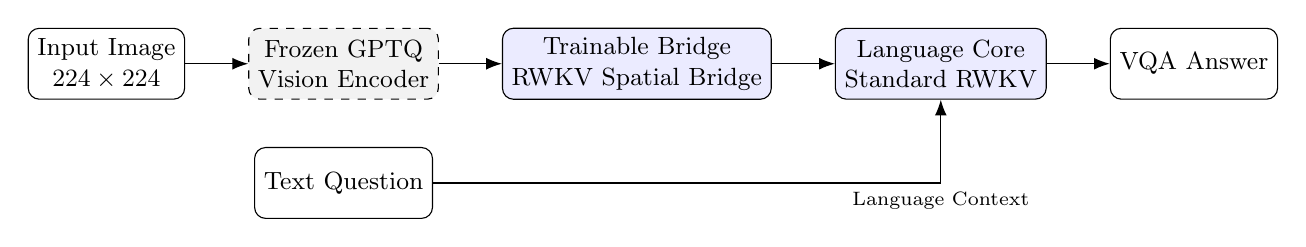
\begin{tikzpicture}[
      node distance=6mm and 8mm,
      box/.style={draw, rounded corners, align=center, minimum height=0.9cm, font=\small},
      frozen/.style={box, dashed, fill=gray!10},
      trainable/.style={box, fill=blue!8},
      arr/.style={-{Latex[length=2mm]}}
    ]
    \node[box] (img) {Input Image\\$224\times224$};
    \node[frozen, right=of img] (enc) {Frozen GPTQ\\Vision Encoder};
    \node[trainable, right=of enc] (bridge) {Trainable Bridge\\RWKV Spatial Bridge};
    \node[trainable, right=of bridge] (core) {Language Core\\Standard RWKV};
    \node[box, right=of core] (ans) {VQA Answer};
    \node[box, below=of enc] (q) {Text Question};

    \draw[arr] (img) -- (enc);
    \draw[arr] (enc) -- (bridge);
    \draw[arr] (bridge) -- (core);
    \draw[arr] (core) -- (ans);
    \draw[arr] (q.east) -| node[below]{\scriptsize Language Context} (core.south);
  \end{tikzpicture}
  \caption{Proposed unified RWKV pipeline. Visual inputs are extracted offline and mapped into
  a recurrent language state machine to enforce a strict sub-100MB footprint.}
  \label{fig:pipeline}
\end{figure}

\section*{Background \& Related Work}

Our project brings together two main ideas: connecting different types of data (vision and
text) and making neural networks run much faster without losing performance. In traditional
setups like LLaVA, a simple linear layer connects a frozen image model to a text model (Liu et
al., 2023). While this is easy to code, it scales poorly because every single image patch gets
sent to the text model, creating a massive data bottleneck. To fix this, models like Flamingo
introduced the Perceiver Resampler, which acts like a smart funnel to squash a large grid of
visual features into a tiny, fixed set of text tokens (Alayrac et al., 2022).

On the language side, standard Transformers are great but they have a massive flaw: they get
slower and take up way too much memory as your input text gets longer. This is why we are using
RWKV, an architecture that trains fast like a Transformer but acts like a lightweight Recurrent
Neural Network (RNN) during inference, meaning its memory footprint stays completely constant
(Peng et al., 2023). To make sure our model fits on a small device, we also look at
quantization methods like GPTQ, which compress heavy model weights into tiny 8-bit integers
without destroying the model's accuracy (Frantar et al., 2023).

\section*{Data Processing}

We are using the standardized VQA v2.0 dataset to train and test our model (Goyal et al.,
2017). Because our model has a strict 100MB limit, we cannot feed it raw, noisy data, so we
perform two major data-cleaning steps. First, human beings answer VQA questions completely
freely, creating thousands of unique text responses. If our model had to learn how to generate
every possible English phrase from scratch, the final text layer alone would take up over 100MB
of storage. To solve this, we find the top-1000 most common answers (like ``yes'', ``no'',
``red'', ``cat'') and turn the project into a 1000-choice multiple-choice problem. Any training
example with a rare, unique answer is dropped.

Second, we resize and normalize all images to a standard $224\times224$ resolution. Instead of
passing these images through our vision encoder during every single training run, we pass them
through the frozen encoder once offline and cache the resulting feature tensors locally. This
saves massive amounts of GPU time, allowing us to focus our training compute entirely on
learning the weights of our custom bridge and text model.

\section*{Architecture}

Our architecture is split into three clean parts, keeping our learning focused entirely on the
interface between vision and text while holding a strict sub-100MB footprint:

\textbf{1. Vision Encoder.} We use a pretrained MobileNetV3 model that is frozen and compressed
down to 8-bit integer precision using GPTQ (Frantar et al., 2023). Because it is frozen, it
takes up zero training compute and acts purely as an offline feature collector.

\textbf{2. Trainable Bridge.} This is where our main innovation happens. We build a specialized
RWKV spatial compressor layer. It processes the visual feature map sequentially as a linear
token track and compresses them down into a tight package of language-aligned tokens without
the overhead of heavy cross-attention matrices.

\textbf{3. Language Backbone \& Loss.} The visual tokens and the text question are fed into a
lightweight RWKV language network, which processes tokens sequentially to eliminate the heavy
math overhead of standard Transformers within our tight 100MB limit (Peng et al., 2023). To
train the model on our 1000-choice vocabulary target, we will use a standard Cross-Entropy Loss
function, which penalizes incorrect category predictions and guides the network to select the
right text answer.

\section*{Baseline Model}

To prove that our pure RWKV approach actually works, we will compare it against a standard,
naive integration baseline. The baseline model will use the exact same frozen MobileNetV3
vision encoder. However, instead of our custom RWKV compression bridge and our lightweight RWKV
text core, the baseline will use a basic Linear Projector layer fed directly into a standard,
unshared Transformer model. This creates a clean control group, allowing us to definitively
check whether our unified RWKV design delivers a better accuracy-to-size tradeoff on the VQA
task.

\section*{Ethical Considerations}

The VQA v2.0 dataset uses images from COCO, which contain real-world scenes that carry implicit
cultural and societal biases. Because our model relies on aggressive parameter compression
under 100MB, it is highly prone to stereotyping. When a network lacks the capacity to store
nuanced visual details, it easily falls back on learned text shortcuts rather than extracting
genuine visual evidence. Additionally, while our model lowers the carbon footprint required for
edge deployment, the iterative training process still consumes GPU compute, which we actively
minimize by using offline feature caching.

\newpage
\section*{References}
Jean-Baptiste Alayrac et al. Flamingo: a visual language model for few-shot learning. In
\emph{Advances in Neural Information Processing Systems}, 2022.

Elias Frantar, Saleh Ashkboos, Torsten Hoefler, and Dan Alistarh. Gptq: Accurate post-training
quantization for generative pre-trained transformers. In \emph{International Conference on
Learning Representations}, 2023.

Yash Goyal, Tejas Khot, Douglas Summers-Stay, Dhruv Batra, and Devi Parikh. Making the v in vqa
matter: Elevating the role of image understanding in visual question answering. In
\emph{Proceedings of the IEEE Conference on Computer Vision and Pattern Recognition}, 2017.

Haotian Liu, Chunyuan Li, Qingyang Wu, and Yong Jae Lee. Visual instruction tuning. In
\emph{Advances in Neural Information Processing Systems}, 2023.

Bo Peng et al. Rwkv: Reinventing rnns for the transformer era. In \emph{Empirical Methods in
Natural Language Processing}, 2023.

\end{document}
